\section{Community Informed Graph Embeddings}
\label{sec: coins}

% \addcontentsline{toc}{section}{Community Informed Graph Embeddings}

In this section we present a new method, called COINs for \textbf{CO}mmunity \textbf{IN}formed graph embedding\textbf{s}, to enhance the efficiency of knowledge graph models for link prediction and conjunctive query answering. COINs uses a community-detection-based graph data augmentation and a two-step prediction pipeline: we first achieve node localization through community prediction, and subsequently, we further localize within the predicted community. We establish theoretical criteria to evaluate our method in our specific context and establish a direct expression of the reduction in time complexity. We empirically demonstrate an important scalability-performance trade-off where for the median evaluation sample we preserve 97.18\% of the baseline accuracy in single-hop query answering, for only 7.52\% of the original computational cost on a single-CPU-GPU machine. 

The work in this section has been accepted for publication as \cite{janchevski_coins_2025}.

\subsection{Motivation}
%Knowledge graphs have recently attracted significant attention from both industry and academia in scenarios that require exploiting large-scale heterogeneous data collections. 
Knowledge graphs are a type of database where the general structure is a \emph{network} of \emph{entities}, their semantic \emph{types}, \emph{properties}, and \emph{relationships}; relations are \emph{flexible} through the use of \emph{abstract classes} to represent real-world data from potentially multiple topical domains~\cite{ehrlinger_towards_2016,hogan_knowledge_2020}. Organizations often use knowledge graphs to catalog and analyze relational data. However, scalability becomes a challenge as the graphs can become very large and require significant computational resources. %This is particularly challenging for smaller organizations.
% Knowledge graphs as a data structure have witnessed numerous applications in a diverse range: journalism, biomedicine, social networks, network security, and telecommunications.

%\textbf{volkan: shorten the paragraph below and merge it with above.}
% Many organizations have internal use for building and maintaining a knowledge graph. The purpose is to neatly organize valuable relational data, analyze it and infer novel information with which to enrich the database.
% This process is referred to as \emph{knowledge graph completion} and it is comprised of solving the tasks of \emph{link prediction} and \emph{query answering} for the knowledge graph. These two tasks can be summarized together as the requirement of building a model that is able to score and rank a set of possible entities/relations (obtained according to the rules of a logical query over the knowledge graph) with regard to relevance. The most common approach in tackling these tasks is to compute suitable \emph{numeric} representations for each graph element, called \emph{graph embeddings}, to use well-understood computational models on them. 
% However, even for smaller organizations, data unlike computational power is not scarce, and the graphs can contain more than hundreds of millions of entities. Therefore, the issue of scalability with respect to both performance and computational cost of knowledge graph inference models arises more frequently in application scenarios as an additional challenge.


Almost all existing scaling approaches involve \emph{splitting the enormous graph into disjoint subsets}, followed by distributed training.
For instance, PyTorch-BigGraph~\cite{lerer_pytorch-biggraph_2019}, and DGL-KE~\cite{zheng_dgl-ke_2020} are distributed-algorithm-system frameworks that can scale the implementation of graph neural networks with distributed execution over billion-scale graphs.
On the other hand, SMORE~\cite{ren_smore_2021} focuses on model parallelization and employs an efficient algorithm for sampling data. CARL-G~\cite{shiao_carl-g_2023} provides similar speed-ups in data sampling to SMORE, but applies only to a non-contrastive setting, and both guarantee acceleration only during training. tf-GNN~\cite{ferludin_tf-gnn_2022} mainly focuses on accelerating the sampling of k-hop neighborhoods of nodes during distributed training.

To this end, we present COINs ({\bf CO}mmunity {\bf IN}formed graph embedding{\bf s}) in a distinct, low resource setting for transductive knowledge graph reasoning model optimization, inference, and evaluation in the contrastive learning setting. We contend that this setting remains elusive to the scalable approaches above, which require a minimum (but still a formidable) level of computational power, and offers new insights to accelerate graph inference. 

In stark contrast, we consider a setting, for instance, where even model evaluation is a major hurdle. Indeed, for the evaluation procedure the state-of-the-art approaches above either apply data parallelization over a large cluster of machines (as for GATNE~\cite{cen_representation_2019}) or use a random subset of the graph (as noted in~\cite{ren_smore_2021}). On the other hand, NodePiece~\cite{galkin_nodepiece_2022} and EARL~\cite{chen_entity-agnostic_2023} are works that, like ours, do not disregard resource efficiency and reduce the overall computational complexity, by admitting a degree of sacrifice in performance. We will argue that, nevertheless, when compared to COINs, they fail to retrieve as much of the baseline performance, only focus on reducing the model size and do not also consider acceleration in inference.

Before explicitly stating our contributions below, we will first establish the background and introduce the preliminaries in the sequel. 


%It is assumed that nevertheless, a minimal cluster size of machines is always available, and any graph partitioning rarely accounts for preserving graph properties. In a low resource availability scenario, even the model's evaluation is a hurdle with big data, which has not been considered in the literature. The evaluation procedure for top-performing knowledge graph representation models was either also sped up with data parallelization over a large cluster of machines (\citet{cen_representation_2019}) or the evaluation metrics are only approximated with a subset of the graph (\citet{ren_smore_2021}).



%Before explicitly stating our contributions below, we will first establish the background and introduce the preliminaries.


 
%all these methods for achieving better scalability are inapplicable to all application scenarios.
%It is assumed that nevertheless, a minimal cluster size of machines is always available, and any graph partitioning rarely accounts for preserving graph properties. In a low resource availability scenario, even the model's evaluation is a hurdle with big data, which has not been considered in the literature. The evaluation procedure for top-performing knowledge graph representation models was either also sped up with data parallelization over a large cluster of machines (\citet{cen_representation_2019}) or the evaluation metrics are only approximated with a subset of the graph (\citet{ren_smore_2021}). 

 
%Our method can be applied to graph embeddings obtained from any model, now used in two steps of query answering prediction, to guarantee the model suffers from much less evaluation cost and with minimal effects on training cost and prediction performance. 

% In the following Section~\ref{sec:background} we give an overview of the relevant background for this text, then in Section~\ref{sec:methodology} we present our proposed method for scalable evaluation, Section~\ref{sec:results} presents and comments on our results, with then Section~\ref{sec:conclusion} briefly concluding.
\vspace{-3mm}
\subsection{Background}
\label{sec:background}
\subsubsection{Problem and Challenges}

\begin{figure}[t!]
    \centering
    \includegraphics[width=0.75\textwidth]{figures/coins/query\_structures.pdf}
    \caption[Various possible computational graph structures of conjunctive knowledge graph queries.]{Various possible computational graph structures of conjunctive knowledge graph queries. Blue nodes indicate query anchors/inputs, green ones are their answers, while the rest are intermediate results. Solid edges represent relation projections, dashed edges represent intersection operations.}
    \label{fig:query_structures}
\end{figure}

Performing knowledge graph inference requires solving link prediction and query answering. Given a dataset of entity-relation-entity triplets, labeled positive or negative according to whether they have originated from the knowledge graph or not, link prediction involves predicting these labels. 

On the other hand, given a list of logical queries extracted from the knowledge graph, the query answering task requires ranking for \emph{each} query \emph{all} of the entities in the graph according to how likely they are to be its correct answer. Thus compared to link prediction, this task is much more computationally complex, as the largest contributor to the number of model inference calls is the size of the graph. Our work aims to reduce this factor significantly.

%One can observe that the query answering task, even in the simplest, single-hop case, entails evaluating the link prediction model as many times as the size of the entire set of entities, for \emph{every} evaluation data sample. On a single machine, this computationally intensive task will incur time complexity proportional to $O\of{N \abs{V}}$, the number of node embeddings required to be computed during evaluation, where $N$ is the number of evaluation samples. Other factors are model-dependent, but in all cases, the size of the node set $\abs{V}$, i.e., the graph size, is the largest contributor. Thus, our work aims to reduce this factor significantly.

% Given an evaluation knowledge graph triplet $\of{h, r, t} \in E_R$, the \emph{single-hop query answering task} entails scoring all possible answers $\hat{t} \in V$ to the query $\of{h, r}$ w.r.t. how probable they are as relations in the knowledge graph, then ranking the answers according to these scores, with the goal that for the best model the true triplet $\of{h, r, t}$ is scored the highest, i.e. has \emph{rank} equal to 1. For this work, we define the rank of a score as the index of the descending order statistic with a value equal to the score, consistent with previous work. 

% With this classical evaluation procedure, we can easily deduce that on a single machine, this is a computationally intensive task with time complexity proportional to $O\of{N \abs{V} D}$, where $N$ is the number of evaluation samples and $D$ is the embedding dimension. Other factors are model-dependent, but in all cases, the size of the node set $\abs{V}$, i.e., the graph size, is the largest contributor. Thus, our work aims to reduce this factor significantly.

\subsubsection{Preliminaries}
% \begin{definition}
% A \textbf{finite graph} $G$ is defined as the ordered pair of two finite sets, $G=\of{V, E}$ where:
% \begin{itemize}
% \item $V=\offf{v_1, \dots, v_N}$ is a finite set of elements, which are referred to as \textbf{nodes};
% \item $E$ is a finite set of elements referred to as \textbf{edges}, where an edge is defined as an ordered pair of nodes: $E=\offf{\of{v_i,v_j} \mid v_i,v_j \in V}$.
% \end{itemize}
% For this text, we will accept the terms \textbf{graph} and \textbf{network} to be equivalent.
% \end{definition}

% \begin{definition}
% Relevant computable graph properties include:
%     \begin{itemize}
%         \item The \textbf{neighbourhood} of a node $v$ is defined as the set of nodes $v$ is directly connected to with an edge: $N\of{v}=\offf{u \mid u\in V, \of{v,u} \in E \vee \of{u,v} \in E }$, while $v$'s \textbf{degree} is the size of its neighbourhood: $deg\of{v}=\abs{N\of{v}}$;
%         \item A \textbf{path} in a graph $G=\of{V, E}$ is a sequence of nodes $v_1,\dots,v_M \in V$ in which every pair of consecutive nodes are connected by an edge: $\forall i \in \offf{1,\dots, M-1},\of{v_i,v_{i+1}}\in E$;
%         \item Given a graph $G = \of{V, E}$, a \textbf{random walk} of length $L$ is a realisation of a discrete stochastic process $\offf{V_i}_{i=1}^L$ where $V_1$ is a random variable with support $V$ and probability mass function $\lambda$, $\sum_{v \in V}{\lambda\of{v}}=1$, while $\forall t\in \offf{2,\dots,L}$, $V_t$ is a random variable with support $N\of{V_{t-1}}$ and probability mass function $\mu_t$, $\sum_{u \in N\of{V_{t-1}}}{\mu_t\of{u}}=1$. Sampling random walks from a graph is a way of converting the graph into a set of path sequences, from which much richer information can be extracted, such as multi-hop connections and node-context pairs.
%     \end{itemize}
% \end{definition}

Mathematically we can represent knowledge graphs with AMHENs:
\begin{definition}
An \emph{Attributed Multiplex HEterogeneous Network (AMHEN)} is a graph where each entity (node) in a set $V$ has attributes and each relation (edge) in a set $E$ has a type label~\cite{liu_ahng_2019,cen_representation_2019}. 

Formally, first, a finite set of \emph{relation types} is defined $R = \offf{r_1,r_2,\dots}$, and the edge labeling is represented through the mathematical relation $E_R \subseteq V \times R \times V$, called the \emph{set of relation triplets}:  $E_R = \offf{\of{h,r,t} \mid h,t \in V, \of{h,t} \in E, r \in R}$. Entity/node attributes can be collected e.g. in a matrix $\mathbf{X} \in \mathbb{R}^{\abs{V} \times F}$, with $F$ as the feature dimension. 

Usually, the nodes $h$ and $t$ in the triplets are referred to as the \emph{head} and \emph{tail} of the relations, respectively. The attributed multiplex heterogeneous network is the new collection $\of{V, E_R, R, \mathbf{X}}$.
\end{definition}

\begin{definition}
    A \emph{query} of the knowledge graph $G=\of{V, E_R, R, \mathbf{X}}$ is the collection $q=\of{\mathcal{A}_q, G_q}$ of a set $\mathcal{A}_q \subseteq V$ of \emph{anchor} (input) entities and $G_q: \mathcal{A}_q \to \mathcal{P}\of{V}$, a mapping visualized via a \emph{computational graph} in the form of a DAG informing how to obtain \emph{answer} entities to the query starting from the anchors, where during this process all of the nodes in $q$ get labeled with sets of entities from $V$. 
    
    In the special case of \emph{conjunctive logical queries}, the edges in $q$ represent either \emph{relation projection} operations $P: \mathcal{P}\of{V} \times R \to \mathcal{P}\of{V}$ (map head to tail along a relation) or \emph{intersection} operations $I: \mathcal{P}\of{\mathcal{P}\of{V}} \to \mathcal{P}\of{V}$ (classical $\cap$), specializing the query mapping as $G_q\of{\mathcal{A}_q;P,I}$~\cite{ren_query2box_2020}.
    \label{def:query}
\end{definition}
Figure~\ref{fig:query_structures} visualizes the computational structures of the conjunctive queries we considered. To give an example of the notation from Definition~\ref{def:query}, the general form of an ip-type conjunctive query $q$ has: $$\mathcal{A}_q=\offf{v_1,v_2}, G_q\of{\offf{v_1,v_2}}=P\of{I\of{\offf{P\of{\offf{v_1},r_1},P\of{\offf{v_2},r_2}}},r_3},$$
where $v_1,v_2 \in V, r_1,r_2,r_3 \in R$ are any entities and relations from $G$.

Graphs are discrete structures, while the majority of machine learning models work exclusively with real-valued continuous inputs. Therefore, we have to construct a mapping from the graph elements to a numeric vector space, such that the output vectors encode the graph structure in the form of algebraic constraints.
\begin{definition}
Given a knowledge graph $G = \of{V, E_R, R, \mathbf{X}}$, in general one defines a \textit{knowledge graph embedding model}~\cite{ji_survey_2022,liang_survey_2024,ren_query2box_2020} as the collection of an entity embedding model $g_V: V \to \mathcal{E}$, relation embedding model $g_R: R \to \mathcal{R}$, relation projection embedding model $g_P: \mathcal{E} \times \mathcal{R} \to \mathcal{E}$, intersection embedding model $g_I: \mathcal{\mathcal{E}}^{\mathbb{N}} \to \mathcal{E}$ and a scoring function $f: \mathcal{E} \times \mathcal{E} \to \mathbb{R}$, all potentially parametrized. Outputs $\mathbf{v} = g_V\of{v}, \mathbf{r} = g_R\of{r}, \mathbf{q}, \mathbf{a}, \dots$ are referred to as \emph{embeddings}. Most often $\mathcal{E}, \mathcal{R} \subseteq \mathbb{R}^D$ or $\mathbb{C}^D$, where $D$ is the \emph{embedding dimension}. 
\end{definition}

Most embedding models are optimized using a contrastive modification of the scoring function:
\begin{definition}
\label{def:contrastive_loss}
    Given the model's scoring function $f$ and the embedding representation of a single \emph{positive} query-answer pair $\of{q, a}$ and a set of $m$ \emph{negative examples} $\offf{a'_i}_{i=1}^{m} \subseteq V \setminus \offf{a}$ (wrong answers to the query), the \emph{contrastive learning loss} terms and final value take the common form ($\sigma$ denoting the sigmoid function):
    \begin{align}
    \begin{aligned}
    \label{eq:contrastive_loss}
        \tilde{\mathcal{L}}\of{\mathbf{q}, \mathbf{a}, y}&=-\log{\sigma{\of{y \cdot f\of{\mathbf{q},\mathbf{a}}}}}\\
        \mathcal{L}\of{\mathbf{q}, \mathbf{a}, \offf{\mathbf{a}'_i}_{i=1}^{m}}&=\tilde{\mathcal{L}}\of{\mathbf{q}, \mathbf{a}, 1} + \frac{1}{m}\sum_{i=1}^{m}{\tilde{\mathcal{L}}\of{\mathbf{q}, \mathbf{a}'_i, -1}}
        \end{aligned}
    \end{align}
\end{definition}

\begin{definition}
    Given a dataset $\mathcal{D}=\offf{\of{h_i, r_i, t_i}}_{i=1}^{N}$ of head-relation-tail triplets and labels $\offf{y_i}_{i=1}^{N}$ indicating whether each triplet was extracted from the knowledge graph or randomly formed, a \emph{link predictor} $\ell: V \times R \times V \to \mathbb{R}$ is a model that aims to predict the label $y_i$ of each triplet $\of{h_i,r_i,t_i}$ by scoring it according to how likely it is to have originated from the knowledge graph.
\end{definition}

% Link predictors are commonly composed of entity-relation embedding models, in order to obtain high-quality feature vectors to pass onto a classifier. 

\begin{definition}
    Given a dataset $\mathcal{D}=\offf{\of{q_i, a_i}}_{i=1}^{N}$ of query-answer pairs extracted from the knowledge graph, \emph{query answering} entails predicting the answer entity $a_i$ given the query information $q_i$ as input. Classically, this is operationalized by forming the set $\hat{\mathcal{D}}_i=\offf{\of{q_i, v}}_{v \in V}$ by combining the query with every possible answer, then the predicted answer is the one that maximizes a scoring model: $\hat{a}_i = \argmax_{v \in V}{S\of{q_i,v}}$.
\end{definition}

\subsubsection{Contributions}
%\textbf{Volkan: Typically, you state the explicit contributions here then explain later on. I currently do not see a clear ``contribution" statement(s).}
Most previous work on knowledge graph inference acceleration~\cite{lerer_pytorch-biggraph_2019,zheng_dgl-ke_2020,ren_smore_2021} focuses on \emph{model-free} solutions relying on hardware and software for distribution and parallelization. Few \emph{model-based} approaches exist that do take resource limitations into account, balancing the model's computational cost with performance, with benefits scaling up with graph size instead of number of compute units.

NodePiece~\cite{galkin_nodepiece_2022} and EARL~\cite{chen_entity-agnostic_2023} propose accelerating knowledge graph prediction tasks by reducing the total number of embedding parameters required. This is done by selecting only certain \enquote{reserved} entities to be a part of a vocabulary $\mathcal{T} \subseteq V$, then only pre-computing the vocabulary embeddings. Embeddings for non-vocabulary entities must be obtained on the spot by selecting for each of them $\tau$ reserved nodes from the vocabulary (via a specific assignment rule) and then re-encoding the sequence of the $\tau$ embeddings. 

Both works thus require at least $\abs{\mathcal{T}} + \tau\of{\abs{V}-\abs{\mathcal{T}}}N$ embedding computations during evaluation, many times larger than the baseline cost of $\abs{V}N$.

On the other hand, our contributions can be summarized as follows: %(I) COINs are a \emph{model-based} approach that performs a novel integration of \emph{community structure information} into optimization and inference, to achieve significant acceleration even with limited resources; and (II) The acceleration potential is exactly derived, with theoretical and empirical arguments for which community structures are optimal.
\begin{enumerate}[I.]
    \item COINs are a \emph{model-based} approach that introduces a novel integration of \emph{community structure information} into optimization and inference to achieve significant acceleration even with limited resources, and balancing speed-up in the best way with baseline performance retrieval and model size;
    \item We derive upper and lower bounds for the total number of embeddings that must be computed during evaluations. By being community-adaptive, our algorithm operates near the lower bound, thereby achieving the best possible speed-ups in practice during evaluation. 
    
    %The acceleration potential is exactly derived, with theoretical and empirical arguments for which community structures are optimal.
\end{enumerate}


\subsubsection{Scalable query answering evaluation}
 Assume that we possess a mapping $c: V \to \mathcal{C}$, assigning knowledge graph entities into one of $\abs{\mathcal{C}} = K \leq \abs{V}$  groups, similar to some previous work~\cite{lerer_pytorch-biggraph_2019,zheng_dgl-ke_2020}. 
 % Instead of only distributing the model training according to this mapping, if it has certain desirable properties, one can utilize it to speed up query answering evaluation as well, through an alternative two-step procedure: 
With $c$ we construct an alternative two-step query answering procedure:
 \begin{enumerate}
     \item Map the input $\of{q, a}$ to a group-level query-answer pair $\of{q^{\of{C}}, c\of{a}}$, and predict $c\of{a}$ by scoring all $K$ possible answer groups;%, where $q^{\of{C}} = \of{\off{c\of{v}}_{v \in \mathcal{A}_q},G_q}$;
     \item Search for the correct answer $a$ only among the entities $\hat{a}$ with $c\of{\hat{a}}=c\of{a}$.
 \end{enumerate}
 % Note that with this new procedure, two scoring models are required, one for each level of prediction, and the performance of the second prediction depends on the first. 
 % However, we now have the potential to greatly reduce the number of model evaluations required, without a large effect on the original evaluation performance, if the mapping $c$ satisfies conditions that we will motivate in the following paragraphs.
% In the following paragraphs, we will show the conditions $c$ must satisfy to obtain our guarantees.

\subsubsection{Optimal partition structure}

First note that the mapping $c$ induces a \emph{disjoint partition} of the entity set $V$. Namely, if we construct the sets $$C_k = \offf{v \in V \mid c\of{v}=k}, k \in \mathcal{C},$$ then $\bigcup_{k=1}^{K}{C_k}=V$ and $\forall i,j \in \mathcal{C},i \neq j, C_i \cap C_j = \emptyset$. 

By analyzing in detail the computational complexity of our new evaluation method, one can easily assess the quality of any such disjoint partition. Proposition~\ref{proposition:complexity} provides our main result. 

\begin{proposition}
\label{proposition:complexity}
Let $\abs{C_k}$ denote the size of node group $k$ and $N_k^{\text{test}}=\abs{\offf{\of{q, a} \in \mathcal{D}_{\text{test}} \mid c\of{a}=k}}$ denote the number of evaluation samples with query answers in node group $k$. The number of query embedding vectors computed in total during evaluation has the following form and bounds:
\begin{equation}
\label{eq:complexity_and_bounds}
2 N \sqrt{\abs{V}} \leq \sum_{k=1}^{K}{\of{K+\abs{C_k}}N_k^{\text{test}}} \leq N \of{\abs{V} + 1} 
\end{equation}
\end{proposition}
The proof is available in Appendix~\ref{sec:appendix_proofs}.
    
% We can prove a quick intuitive result about disjoint partitions:
% \begin{proposition}
% \label{proposition:average_community_size}
% Given a graph $G=\of{V, E}$, assume that a disjoint partitioning of $V$ into $K=O\of{\abs{V}^p}$, groups was obtained, with naturally $p \in \of{0, 1}$. Then no matter the partition assignment, the average group size will be $O\of{\abs{V}^{1-p}}$.
% \end{proposition}
% \begin{proof}
%     Observe that simply: $\frac{1}{K}\sum_{k=1}^{K}{C_k} = \frac{1}{K}\abs{V}=O\of{\abs{V}^{-p} \cdot \abs{V}}=O\of{\abs{V}^{1-p}}$.
% \end{proof}

% Now, the time complexity of the first, node group prediction step of the new evaluation procedure, is proportional to the number of groups $K$, as this is the number of model evaluation steps required, and therefore it is on the order of $\Theta\of{\abs{V}^{p} D}$. On the other hand, the second step on average requires as many model evaluations as the average group size. 
% From proposition~\ref{proposition:average_community_size} however, we know that for this disjoint partitioning of the node set the average group size will be on the order of $O\of{\abs{V}^{1-p}}$, thus the complexity of the second step amounts to $\Theta\of{\abs{V}^{1-p} D}$ and the total cost of the new evaluation procedure is thus: $\Theta\of{N \off{\abs{V}^{p} + \abs{V}^{1-p}} D}$. 
% From Proposition~\ref{proposition:average_community_size} however, we know the expected average group size, and thus the complexity of the second step amounts to $\Theta\of{\abs{V}^{1-p} D}$ and the total cost of the new evaluation procedure is thus: $\Theta\of{N \off{\abs{V}^{p} + \abs{V}^{1-p}} D}$. 
% But, by choosing a different $c$, one has the option to optimize the value of $p$, and the following Proposition~\ref{proposition:min_evaluation_cost} argues which value minimizes our overall cost:
% \begin{proposition}
%     \label{proposition:min_evaluation_cost}
%     With $p=\frac{1}{2}$, one achieves the minimal evaluation cost of $\Theta\of{N \sqrt{\abs{V}} D}$.
% \end{proposition}
% \begin{proof}
%     Let $g\of{p} = \abs{V}^{p} + \abs{V}^{1-p}$. Then note that $g'\of{p} = \log{\abs{V}}\of{\abs{V}^{p} - \abs{V}^{1-p}}$. From this, we find the only critical point of $g$ in $\of{0, 1}$: $\abs{V}^{p} - \abs{V}^{1-p} = 0 \Leftrightarrow p = 1-p \Leftrightarrow p = \frac{1}{2}$. As $g''\of{\frac{1}{2}} = 2\log^{2}{\abs{V}}\sqrt{\abs{V}} > 0$, $p^* = \frac{1}{2}$ indeed is the minimizer.
% \end{proof}

\subsubsection{Query locality}
The lower bound of equation \eqref{eq:complexity_and_bounds} above states that it is possible to achieve a $\sqrt{\abs{V}}$ dependence in evaluations while the scalable approaches we have discussed so far have a linear dependence on ${\abs{V}}$. 
%The possibility of quadratically reducing the overall computation time is grounds for sufficient motivation to obtain a partitioning that splits the node set into $K=O\of{\sqrt{\abs{V}}}$ equally sized pieces, as its first important property. 
However, to minimally affect the baseline performance, we must consider the partitioning quality from the perspective of preserving the relational structure. 

What previous works often fail to consider is that an arbitrary assignment might be \emph{arbitrarily non-local}. Formally, if we construct the set $$V^*\of{c}=\offf{v \in V \mid \exists \of{u,r}, E_R \cap \offf{\of{v,r,u}, \of{u, r, v}} \neq \emptyset, c\of{u} \neq c\of{v}}$$ of entities that participate in between-group relations, then we must have both minimal $\abs{V^*\of{c}}$ as well as minimal total evaluation cost (Proposition~\ref{proposition:complexity}). 

In this case, the search for the true answer to a query will be most often localized to a small neighborhood in the knowledge graph, a significantly easier problem. Equivalently, one prefers a mapping $c$ such that more relations are present \emph{within} the entity sets $C_k$ than \emph{between} the sets. 

Unfortunately, achieving good localization is an NP-hard problem, but research in the fields of \emph{community detection} and \emph{minimal cuts} for graphs have yielded extremely efficient heuristic algorithms. 

Such is the Leiden algorithm for community detection~\cite{traag_louvain_2019}, the current state-of-the-art, based on heuristic maximization of the Constant Potts Model~\cite{traag_narrow_2011} version of the modularity score~\cite{blondel_fast_2008}, with further manual refinement to guarantee well-connected communities. The single \enquote{resolution} hyperparameter of the algorithm is the only degree of freedom controlling the community assignment quality. To this end, our work represents a novel application of Leiden communities to knowledge graph inference. 

On the other hand, the METIS algorithm for graph partitioning~\cite{karypis_fast_1998}, employed also in~\cite{zheng_dgl-ke_2020}, strives towards minimal graph cuts. For some experiments, we considered it as an alternative to Leiden to estimate the effect of the choice of graph-splitting method.

\subsection{Methodology}
\label{sec:methodology}

\subsubsection{Community detection}

Given a knowledge graph $\of{V, E_R, R, \mathbf{X}}$, the first step we employ is to execute the Leiden community detection algorithm to obtain a good node-to-community mapping $c: V \to \mathcal{C}$. 

% We observed that, in practice, if the graph is sufficiently sparse, i.e., $\abs{E_R} \ll \abs{R} \cdot \abs{V}^2$, with the resolution parameter of the algorithm simply set to $\frac{1}{\abs{V}}$ one achieves decent performance without the need for further validation. Obtaining quality community assignments for dense graphs, however, is very challenging, and validation of the resolution hyperparameter is recommended. Additionally, one can merge very small weakly connected components into larger communities to achieve a better balance of community sizes. 

For our COINs technique, based on the obtained community assignment map $c$ we extract further discrete information of great utility for efficient training and evaluation. $c$ coarsens $\of{V, E_R}$ into a \emph{community-level interaction graph}: $$V^{\of{C}} = \mathcal{C}, E^{\of{C}}_R = \offf{\of{c\of{u},r,c\of{v}} \mid \of{u,r,v} \in E_R}.$$%
In addition, one can compute the \emph{inter-community mapping} $z^*: V \to V_{\omega}^*$:
$$z^*\of{v}=\begin{cases} v, & \text{ if } v \in V^* \\ \omega, & \text{ otherwise} \end{cases}$$where $V_{\omega}^* = V^* \cup \offf{\omega}$ and $\omega$ is a padding node representing all nodes in $V \setminus V^*$.

\subsubsection{COINs training \& evaluation}

% As we introduced previously, state-of-the-art knowledge graph embedding models and methods for achieving better scalability are inapplicable for all scenarios, either since node partitions are sub-optimal or intermediate computation variables are unoptimized for single-machine computation. As such, in the following paragraphs, the proposed COINs knowledge graph representation technique is presented, facilitating the community-based graph data augmentations to their fullest.

Let $\mathcal{F}$ denote the class of knowledge graph embedding models whose scalability we wish to improve, and $\tilde{\mathcal{L}}: \mathcal{E} \times \mathcal{E} \times \offf{-1,1} \to \mathbb{R}$ be the per-sample contrastive loss term minimized during training such models (eq. \eqref{eq:contrastive_loss}). 
% \newpage

COINs requires the optimization of the following models sampled from $\mathcal{F}$:
\begin{itemize}
    \item {Community-level embedders} 
    
    $g_V^{\of{C}}: \mathcal{C} \to \mathcal{E}, g_R^{\of{C}}: R \to \mathcal{R}, g_P^{\of{C}}: \mathcal{E} \times \mathcal{R} \to \mathcal{E}, g_I^{\of{C}}: \mathcal{E}^{\mathbb{N}} \to \mathcal{E}$;
    \item {Intra-community entity embedders} $g_V^{\of{k}}: C_k \to \mathcal{E}, \forall k \in \mathcal{C}$;
    \item {Inter-community entity embedder} $g_V^{*}: V_{\omega}^* \to \mathcal{E}$. 
    \item {Node-level relation and query embedders} 
    
    $g_R: R \to \mathcal{R}, g_P: \mathcal{E} \times \mathcal{R} \to \mathcal{E}, g_I: \mathcal{E}^{\mathbb{N}} \to \mathcal{E}$
\end{itemize}

Additional parameters are: a {node feature embedding matrix} $\mathbf{W} \in \mathbb{R}^{D \times F}$ and {node/relation embedding aggregation weights} $\mathbf{w} \in \mathbb{R}^{3}, \mathbf{w}_R \in \mathbb{R}^{2}$.

\begin{algorithm}[H]
    \caption{Base knowledge graph representation}
    \label{algorithm:baseline}
    \begin{algorithmic}[1]
    \STATE{\textbf{input} $\of{q, a}$, $y \in \offf{-1,1}$}
    \STATE{$\mathbf{R}\gets\off{g_R\of{r}}_{r \in R}$}
    \STATE{$\mathbf{a} \gets g_V\of{a}, \mathbf{A}\gets\off{g_V\of{v}}_{v \in \mathcal{A}_{q}}$}
    \STATE{$\mathbf{q} \gets G_{q}\of{\mathbf{A};\of{\mathbf{R},g_P},g_I}$}
    \STATE{\textbf{return} $\tilde{\mathcal{L}}\of{\mathbf{q}, \mathbf{a}, y}$}
    \end{algorithmic}
\end{algorithm}

 Algorithm~\ref{algorithm:baseline} presents the baseline inference steps required, Algorithm~\ref{algorithm:coins} details the knowledge graph query representation steps for COINs, utilizing the constructed sub-models, while Figure~\ref{fig:community_preprocessing} provides a visualization of our community-based preprocessing and query representation on a small example. 

This new construction has several desirable properties unlike the baseline: 
\begin{enumerate}
    \item Queries spanning multiple communities are treated differently, allowing for greater generalization; 
    \item $K + \max{\of{\max_{k=1}^{K}{\abs{C_k}},\abs{V^{*}} + 1}}$ will be the maximum number of entity embeddings to compute for each training iteration instead of the baseline $\abs{V}$, an overall lower time and memory cost;
    \item The community representation learning will be performed jointly with the node-level, due to the softmax-weighted embedding refinement linking them both, allowing for greater adaptivity;
    % \item The final embedding refinement will preserve the convexity of the base model, if it has that property.
\end{enumerate}

% \centerline{
% \begin{adjustbox}{width=\textwidth}%, totalheight=40ex}
% \hfill
% \begin{minipage}{\textwidth}
\begin{algorithm}[H]
% \algsetup{linenosize=\tiny}
% \scriptsize
\caption{COINs knowledge graph representation}
\label{algorithm:coins}
\begin{algorithmic}[1]
\STATE{\textbf{input} $\of{q, a}$, $y \in \offf{-1,1}$, $c:V \to \mathcal{C}$, $z^*: V \to V_{\omega}^*$, $\alpha \in \of{0,1}$}
\STATE{$\mathbf{R}^{\of{C}} \gets \off{g^{\of{C}}_R\of{r}}_{r \in R}, \tilde{\mathbf{R}} \gets \off{g_R\of{r}}_{r \in R}$}
\STATE{$\mathbf{R} \gets \ang{ \mathrm{Softmax}\of{\mathbf{w}_R}, \off{\mathbf{R}^{\of{C}}, \tilde{\mathbf{R}}} }$}
\STATE{$q^{\of{C}} \gets \of{\off{c\of{v}}_{v \in \mathcal{A}_q},G_q}$}
\STATE{$\mathbf{a}^{\of{C}} \gets g^{\of{C}}_V\of{c\of{a}}, \mathbf{A}^{\of{C}} \gets \off{g^{\of{C}}_V\of{k}}_{k \in \mathcal{A}^{\of{C}}_{q}}$}
\STATE{$\mathbf{q}^{\of{C}} \gets G_{q}\of{\mathbf{A}^{\of{C}};\of{\mathbf{R}^{\of{C}},g_P^{\of{C}}},g_I^{\of{C}}}$}
\IF{$\forall v \in q, c\of{v}=c\of{a}$}
\STATE{$\tilde{\mathbf{a}} \gets g^{\of{c\of{a}}}_V\of{a}, \tilde{\mathbf{A}} \gets \off{g^{\of{c\of{a}}}_V\of{v}}_{v \in \mathcal{A}_{q}}$}
\ELSE
\STATE{$\tilde{\mathbf{a}} \gets g^{*}_V\of{z^*\of{a}}, \tilde{\mathbf{A}}\gets\off{g^{*}_V\of{z^*\of{v}}}_{v \in \mathcal{A}_{q}}$}
\ENDIF
\STATE{$\mathbf{a} \gets \ang{\mathrm{Softmax}\of{\mathbf{w}}, \off{\mathbf{W} \mathbf{x}_{a}, \mathbf{a}^{\of{C}}, \tilde{\mathbf{a}}}}, \mathbf{A} \gets \ang{ \mathrm{Softmax}\of{\mathbf{w}}, \off{\mathbf{W} \mathbf{x}_{v}}_{v \in \mathcal{A}_{q}}, \mathbf{A}^{\of{C}}, \tilde{\mathbf{A}} }$}
\STATE{$\mathbf{q}\gets G_{q}\of{\mathbf{A};\of{\mathbf{R},g_P},g_I}$}
\STATE{\textbf{return} $\tilde{\mathcal{L}}_{\text{COINs}}\of{\mathbf{q}, \mathbf{a}, y}=\of{1-\alpha} \tilde{\mathcal{L}}\of{\mathbf{q}^{\of{C}}, \mathbf{a}^{\of{C}}, y} + \alpha \tilde{\mathcal{L}}\of{\mathbf{q}, \mathbf{a}, y} $}
\end{algorithmic}
\end{algorithm} 
% \end{minipage}
% \hfill\mbox{}
% \end{adjustbox}}

\begin{figure}[H]
    \centering
    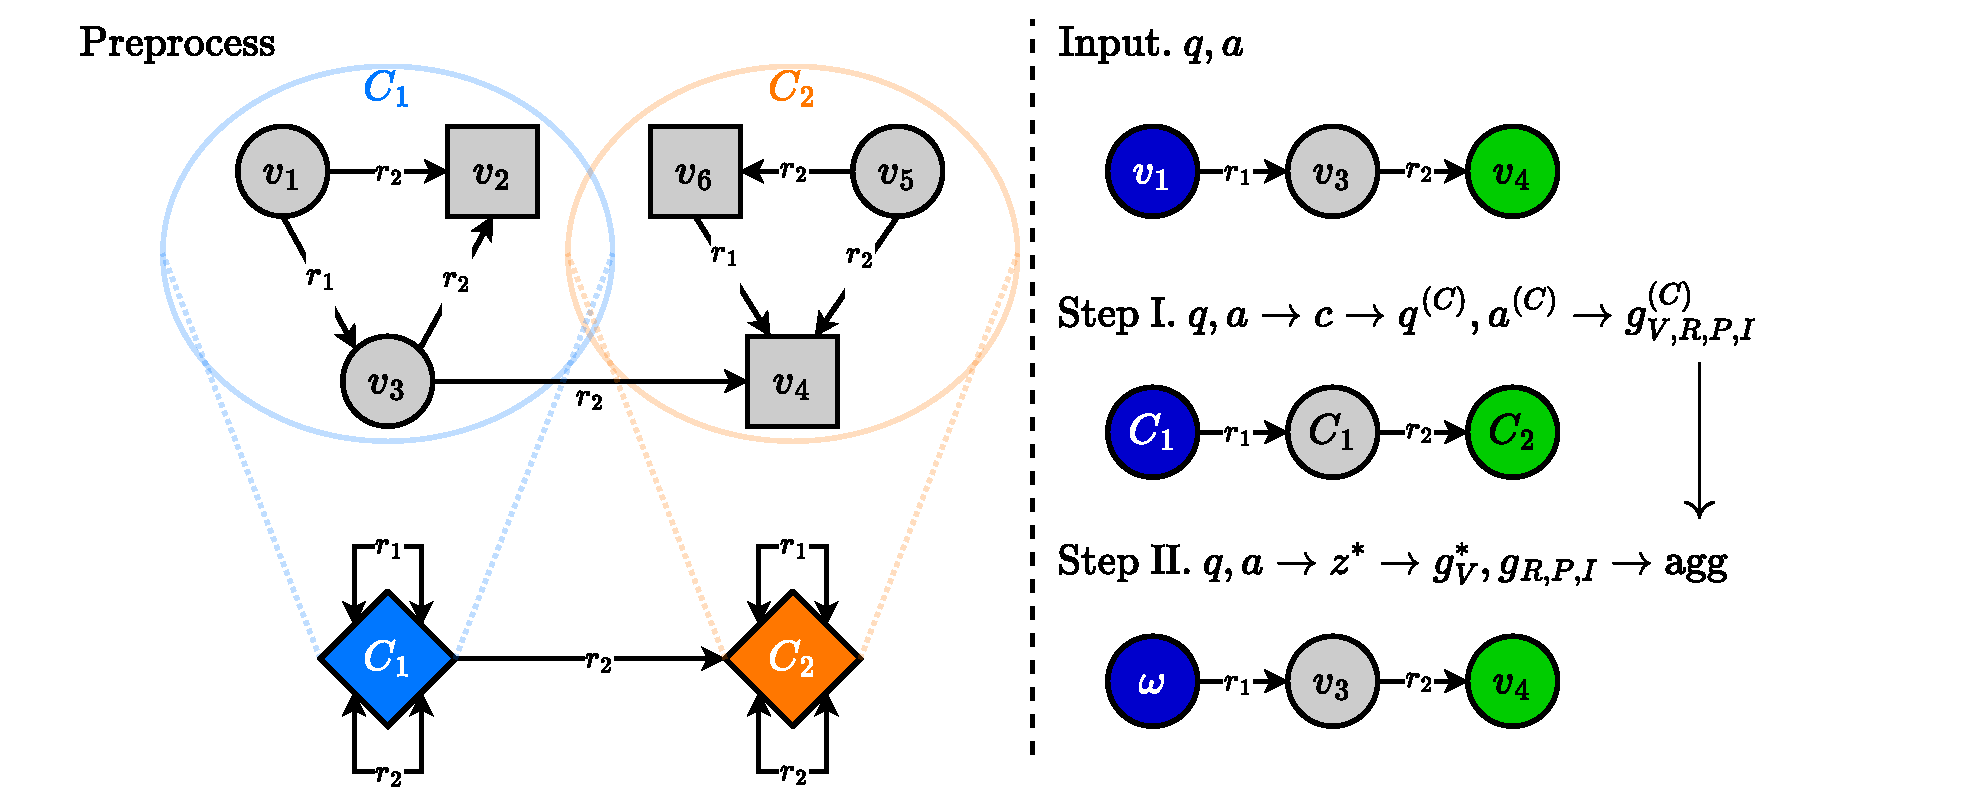
\includegraphics[width=0.75\textwidth]{figures/coins/coins.pdf}
    \caption[Example of a preprocessed knowledge graph and the COINs representation process on an example query.]{Left: example of a preprocessed knowledge graph, showing its transformation into a community-level graph, with $\abs{V}=6, \abs{E_R}=7, T=2, \abs{R}=2, K=2, \abs{V^*}=2$. Right: the COINs representation process on an example inter-community 2p-query of the graph on the left.}
    \label{fig:community_preprocessing}
\end{figure}

Observe that the total number of COINs node embeddings for a graph is $K + \sum_{k=1}^{K}{\abs{C_k}} + \abs{V^*} + 1 = K + \abs{V} + \abs{V^*} + 1$, compared to just $\abs{V}$ node embeddings in the baseline. Thus, using a partitioning that keeps $\abs{V^*} \ll \abs{V}$ has benefits in limiting model size as well. 

Let now $S_C$ denote a learned scoring model for community-level query-answer pairs, obtained after extending the community-level COINs sub-models into a classifier, with $S_V$ the analog for the final node-level query answer scoring. Then, one can implement the proposed novel scalable query answering procedure via Algorithm~\ref{algorithm:scalable_query_answering}. %Note that, all query answering evaluation metrics are aggregates of the predicted \emph{ranks} of the evaluation triplets. %, defined as the index of the descending order statistic of the predicted link scores equal to the score of the true answer triplet. 
% Thus, our evaluation algorithm also must efficiently compute these ranks while taking into account that the node ranking is performed in two steps. 

% \begin{wrapfigure}{R}{0.5\textwidth}
% \begin{minipage}{0.5\textwidth}
% \vspace{-19.85ex}
\begin{algorithm}[H]
\caption{COINs query answering evaluation}
\label{algorithm:scalable_query_answering}
\begin{algorithmic}[1]
\STATE{\textbf{input} test set $\mathcal{D}_{\text{test}}=\offf{\of{q_i, a_i}}_{i=1}^{N}$, scorers $S_C, S_V$}
\FOR{$i \gets 1$ to $N$}
\STATE{$q^{\of{C}}_i \gets \of{\off{c\of{v}}_{v \in \mathcal{A}_{q_i}},G_{q_i}}$}
\STATE{$s_C \gets \off{S_C\of{q^{\of{C}}_i, k}}_{k \in \mathcal{C}}$}
\STATE{$\rho^{\of{i}}_{C} \gets \mathrm{Rank}\of{c\of{a_i},s_C}$}
\STATE{$F_i \gets \sum_{1 \leq j < \rho^{\of{i}}_{C}}{\abs{C_{\mathrm{IndexRank}\of{j,s_C}}}}$}
\STATE{$s_V \gets \off{S_V\of{q_i, v}}_{v \in C_{c\of{a_i}}}$}
\STATE{$\tilde{\rho}^{\of{i}} \gets \mathrm{Rank}\of{a_i,s_V}$}
\STATE{$\rho^{\of{i}} \gets F_i + \tilde{\rho}^{\of{i}}$}
\ENDFOR
\STATE{\textbf{return} $\off{\rho^{\of{i}}}_{i=1}^{N}$}
\end{algorithmic}
\end{algorithm} 
% \end{minipage}
% \end{wrapfigure}


\subsubsection{Tradeoff analysis}

The primary limitation of the COINs evaluation procedure is that incorrect community prediction can result in many nodes being returned as false positives (large $F_i$ term in Algorithm~\ref{algorithm:scalable_query_answering}). This conditional nature of the prediction is the main reason for expecting lower performance compared to the baseline. 

However, as community ranks approach 1, we can much more quickly obtain model predictions with lesser and lesser drawbacks for large graphs. Thus, we prove Proposition~\ref{proposition:condition_applicability}, which quantifies under which conditions the application of COINs is feasible, by theoretically analyzing the tradeoff between the possible scalability benefits and performance losses. 

The general takeaway is that one must \emph{per-community} consider the ratio between acceleration factors and relative error in performance metrics, with specific weight values for aggregating these comparisons to obtain a final conclusion through a simple inequality test.


\subsubsection{Distributed extension}

As previously mentioned, previous work mainly solves the problem of query answering scalability by distributing the knowledge graph embedding model across many compute units. Both data and model parallelism are almost fully achieved in this manner, however the acceleration is always only at best linear with respect to the number of machines available. As such, to scale to very large knowledge graphs a very large cluster of at least hundreds of machines is required. In this part of the thesis, I will suggest how to utilize available computation resources more efficiently through extending COINs to the distributed learning setting.

Namely, the COINs submodel structure naturally permits partial model parallelism in addition to the acceleration incurred from the two-step inference process. The intra-community and inter-community models used during step 2 of the process are by design independent. This is due to the fact that each of those models trains and predicts over a disjoint subset of the knowledge graph edges. As such, Step 2 can be completely parallelized across multiple machines, by assigning for each intra-community or inter-community model a dedicated compute unit. The only unavoidable bottleneck is having to sequentially wait for the community prediction of Step 1 to finish, in order to have the information to which machine a data point needs to be communicated.

The distributed COINs architecture is proposed to be as follows. Let $U$ be a finite set of compute units available to the application, and let $\mathcal{M} \subset \mathcal{F}$ be the full set of COINs submodels. The assignment of COINs models to units will be represented through the mapping $u: \mathcal{M} \to U$. First, select a machine $u^* \in U$ to serve as the \emph{leader} node. The leader performs Step 1, sends and receives data between itself and the other machines to orchestrate Step 2 and perfoms the final aggregation steps. Formally, we fix these assignments:
$$u\of{g_V^{\of{C}}}=u\of{g_R^{\of{C}}}=u\of{g_P^{\of{C}}}=u\of{g_I^{\of{C}}}=u\of{g_R}=u\of{g_P}=u\of{g_I}=u\of{\mathbf{W}}=u\of{\mathbf{w}}=u\of{\mathbf{w}_R}=u^*.$$
Then with this setup, Algorithm \ref{algorithm:coins_distributed} details the distributed version of Algorithms \ref{algorithm:coins}. For easier comparison, I color-highlight the required changes for the distributed extension.

\begin{algorithm}[H]
% \algsetup{linenosize=\tiny}
% \scriptsize
\caption{Distributed COINs knowledge graph representation}
\label{algorithm:coins_distributed}
\begin{algorithmic}[1]
\STATE{\textcolor{blue}{\textbf{on} $u^*$:}}
\STATE{\textbf{input} $\of{q, a}$, $y \in \offf{-1,1}$, $c:V \to \mathcal{C}$, $z^*: V \to V_{\omega}^*$, $\alpha \in \of{0,1}$}
\STATE{$\mathbf{R}^{\of{C}} \gets \off{g^{\of{C}}_R\of{r}}_{r \in R}, \tilde{\mathbf{R}} \gets \off{g_R\of{r}}_{r \in R}$}
\STATE{$\mathbf{R} \gets \ang{ \mathrm{Softmax}\of{\mathbf{w}_R}, \off{\mathbf{R}^{\of{C}}, \tilde{\mathbf{R}}} }$}
\STATE{$q^{\of{C}} \gets \of{\off{c\of{v}}_{v \in \mathcal{A}_q},G_q}$}
\STATE{$\mathbf{a}^{\of{C}} \gets g^{\of{C}}_V\of{c\of{a}}, \mathbf{A}^{\of{C}} \gets \off{g^{\of{C}}_V\of{k}}_{k \in \mathcal{A}^{\of{C}}_{q}}$}
\STATE{$\mathbf{q}^{\of{C}} \gets G_{q}\of{\mathbf{A}^{\of{C}};\of{\mathbf{R}^{\of{C}},g_P^{\of{C}}},g_I^{\of{C}}}$}
\IF{$\forall v \in q, c\of{v}=c\of{a}$}
\STATE{\textcolor{blue}{\textbf{async send} $\of{\mathcal{A}_q, a} \to u\of{g_V^{c\of{a}}}$}}
\STATE{\textcolor{blue}{\textbf{on } $u\of{g_V^{c\of{a}}}$:}}
\STATE{$\tilde{\mathbf{a}}\gets g^{\of{c\of{a}}}_V\of{a}, \tilde{\mathbf{A}} \gets \off{g^{\of{c\of{a}}}_V\of{v}}_{v \in \mathcal{A}_{q}}$}
\STATE{\textcolor{blue}{\textbf{async send} $\of{\tilde{\mathbf{A}}, \tilde{\mathbf{a}}} \to u^*$}}
\ELSE
\STATE{\textcolor{blue}{\textbf{async send} $\of{\mathcal{A}_q, a} \to u\of{g_V^{*}}$}}
\STATE{\textcolor{blue}{\textbf{on } $u\of{g_V^{*}}$:}}
\STATE{$\tilde{\mathbf{a}} \gets g^{*}_V\of{z^*\of{a}}, \tilde{\mathbf{A}} \gets \off{g^{*}_V\of{z^*\of{v}}}_{v \in \mathcal{A}_{q}}$}
\STATE{\textcolor{blue}{\textbf{async send} $\of{\tilde{\mathbf{A}}, \tilde{\mathbf{a}}} \to u^*$}}
\ENDIF
\STATE{\textcolor{blue}{\textbf{on} $u^*$:}}
\STATE{\textcolor{blue}{\textbf{sync wait} $\of{\tilde{\mathbf{A}}, \tilde{\mathbf{a}}}$}}
\STATE{$\mathbf{a} \gets \ang{ \mathrm{Softmax}\of{\mathbf{w}}, \off{\mathbf{W} \mathbf{x}_{a}, \mathbf{a}^{\of{C}}, \tilde{\mathbf{a}}}}, \mathbf{A} \gets \ang{ \mathrm{Softmax}\of{\mathbf{w}}, \off{\mathbf{W} \mathbf{x}_{v}}_{v \in \mathcal{A}_{q}}, \mathbf{A}^{\of{C}}, \tilde{\mathbf{A}} }$}
\STATE{$\mathbf{q} \gets G_{q}\of{\mathbf{A};\of{\mathbf{R},g_P},g_I}$}
\STATE{\textbf{return} $\tilde{\mathcal{L}}_{\text{COINs}}\of{\mathbf{q}, \mathbf{a}, y}= \of{1-\alpha} \tilde{\mathcal{L}}\of{\mathbf{q}^{\of{C}}, \mathbf{a}^{\of{C}}, y} + \alpha \tilde{\mathcal{L}}\of{\mathbf{q}, \mathbf{a}, y} $}
\end{algorithmic}
\end{algorithm} 

The choice on which machine to assign to the inter-community model and each intra-community model is arbitrary, however there exists expectedly an optimal assignment in order to achieve the best scalability benefits. Interestingly, by optimizing the model-to-machine distribution in conjunction with the community sizes, one can achieve a cubic instead of quadratic overall acceleration. Proposition \ref{proposition:complexity_distributed} presents this new result, which extends Proposition \ref{proposition:complexity} to the distributed setting and whose proof I provide in Appendix \ref{sec:appendix_proofs}. The introduced changes to the single-machine computational complexity are highlighted for easier comparison.

\begin{proposition}
\label{proposition:complexity_distributed}
    Let $N_{k,k}^{\text{test}}=\abs{\offf{\of{q, a} \in \mathcal{D}_{\text{test}} \mid \forall v \in q, c\of{v}=c\of{a}=k}}$ denote the number of intra-community evaluation samples with query nodes and answers in node group $k$. The largest number of query embedding vectors computed in parallel during distributed evaluation has the following form and bounds:
\begin{equation}
\label{eq:complexity_and_bounds_distributed}
\frac{3}{2} N \sqrt[3]{2\abs{V}} \leq KN+\textcolor{blue}{\max_{l=1}^{\abs{U}}}{\of{\sum_{k=1}^{K}{\abs{C_k}\off{N_{k,k}^{\text{test}}\textcolor{blue}{\mathbb{I}\of{u\of{g_V^k}=u_l}} + \of{N_k^{\text{test}}-N_{k,k}^{\text{test}}}\textcolor{blue}{\mathbb{I}\of{u\of{g_V^*}=u_l}}}}}} \leq N \of{\abs{V} + 1} 
\end{equation}
\end{proposition}

The proof of the previous results explains that to achieve the best possible cost after parallelization of COINs, we must distribute equally the amount of work each machine will do for Step 2. With integer packet sizes however, this is called the \emph{balanced partition} problem, a known NP-hard variant of the 0-1 Knapsack problem. 

In our case, we have an array of costs $\offf{p_k}_{k=1}^{K+1}=\offf{\abs{C_k}N_{k,k}^{\text{test}}}_{k=1}^{K}\cup\offf{\sum_{k=1}^{K}{\abs{C_k}\of{N_{k}^{\text{test}}-N_{k,k}^{\text{test}}}}}$ that have to be assigned to $\abs{U}$ knapsacks, such that the maximal total amount in one knapsack is minimal. A brute-force algorithm checking all possible assignments would have a worst case cost of $O\of{\abs{U}^{K+1}}$, which is infeasible. There exists an alternative dynamic programming solution with the pseudo-polynomial complexity of $O\of{\of{K+1}S^{\abs{U}-1}}$, where $S$ is the number of unique subset sums in $\offf{p_k}_{k=1}^{K+1}$. However, in practice it is also often infeasible to run for $\abs{U}\geq 3$. Thus, for this problem an inexact greedy algorithm can be preferred, as by simply assigning one-by-one the biggest packet to the least-filled knapsack one very closely approximates the optimal solution, with the much lower computation cost of $O\of{\of{K+1}\log_2{\of{\abs{U}\of{K+1}}}}$. For completeness, in Appendix \ref{sec:appendix_balanced_partition_algs} we provide the pseudocode for the two assignment algorithms.

\subsubsection{Experiment setup}

\paragraph{Integration with knowledge graph representation models}
Due to the universality of our COINs technique for scaling up knowledge graph model evaluation, we can integrate it with many established knowledge graph embedding models, described in Table~\ref{tab:algorithms} below. Each performs contrastive learning, i.e., minimization of equation \eqref{eq:contrastive_loss}. 
\begin{table}[H]
  \caption[Knowledge graph embedding model summary.]{Knowledge graph embedding model summary. Left to right: node \& relation embedding space, embedding parameter constraints, relation projection model, intersection model, score function.}
  \label{tab:algorithms}
  \centering
\begin{adjustbox}{width=\textwidth}
\begin{tabular}{lcccccc}
\toprule
Model & $\mathcal{E}$ & $\mathcal{R}$ & Constraints & $g_P\of{\mathbf{v}, \mathbf{r}}$ & $g_I\of{\off{\mathbf{v}}}$ & $f\of{\mathbf{q}, \mathbf{a}}$ \\
\midrule
\textbf{TransE}~\cite{bordes_translating_2013} & $\mathbb{R}^D$ & $\mathbb{R}^D$ & $\abs{\abs{\mathbf{v}}}=1$ & $\mathbf{v} + \mathbf{r}$ & \textemdash & $\gamma - \abs{\abs{\mathbf{q} - \mathbf{a}}}$ \\
\textbf{DistMult}~\cite{yang_embedding_2014} & $\mathbb{R}^D$ & $\mathbb{R}^D$ & $\abs{\abs{\mathbf{v}}}=1$ & $\mathbf{v} \odot \mathbf{r}$ & \textemdash & $\ang{ \mathbf{q}, \mathbf{a} }$ \\
\textbf{ComplEx}~\cite{trouillon_ComplEx_2016} & $\mathbb{C}^D$ & $\mathbb{C}^D$ & \textemdash & $\mathbf{v} \cdot \mathbf{r}$ & \textemdash & $\text{Re}{\of{\ang{ \mathbf{q}, \bar{\mathbf{a}} }}}$ \\
\textbf{RotatE}~\cite{sun_rotate_2019} & $\mathbb{C}^D$ & $\mathbb{C}^D$ & $\forall d, \abs{\mathbf{r}^{\of{d}}}=1$ & $\mathbf{v} \cdot \mathbf{r}$ & \textemdash & $\gamma - \abs{\abs{\mathbf{q} - \mathbf{a}}}$ \\
 \textbf{KBGAT}~\cite{nathani_learning_2019} & $\mathbb{R}^D$ & $\mathbb{R}^D$ & $\abs{\abs{\mathbf{v}}}=1$ & GAT$_r$~\cite{velickovic_graph_2018} & \textemdash & ConvKB~\cite{nguyen_novel_2018} \\
 \multirow{2}{*}{\textbf{Query2Box}~\cite{ren_query2box_2020}} & \multirow{2}{*}{$\mathbb{R}^{2D}$} & \multirow{2}{*}{$\mathbb{R}^{2D}$} & $\mathbf{v}=\off{\mathbf{v}^{\of{c}}, \mathbf{v}^{\of{o}}}$, & \multirow{2}{*}{$\mathbf{v} + \mathbf{r}$} & $\text{Att}\of{\off{\mathbf{v}^{\of{c}}}},$ & $\gamma - f_{\text{out}}\of{\mathbf{q},\mathbf{a}}  $\\
  &  &  & $\mathbf{v}^{\of{o}} \geq 0$ & & $\text{MinDS}\of{\off{\mathbf{v}^{\of{o}}}}$  & $-\beta f_{\text{in}}\of{\mathbf{q},\mathbf{a}}$  \\
\bottomrule
\end{tabular}
\end{adjustbox}
$\text{Att}\of{\off{\mathbf{v}^{\of{c}}}}=\ang{ \text{Softmax}\of{\text{MLP}\of{\off{\mathbf{v}}}}, \off{\mathbf{v}^{\of{c}}} }$, \\$\text{MinDS}\of{\off{\mathbf{v}^{\of{o}}}} = \min_{\mathbf{u}}{\off{\mathbf{u}^{\of{o}}}} \odot \sigma\of{\text{DeepSets}\of{\off{\mathbf{v}}}}$~\cite{zaheer_deep_2017,hamilton_embedding_2018}, \\
$f_{\text{out}}\of{\mathbf{q},\mathbf{a}} = \abs{\abs{\text{ReLU}\of{\mathbf{a}^{\of{c}} - \mathbf{q}^{\of{c}} - \mathbf{q}^{\of{o}}} + \text{ReLU}\of{\mathbf{q}^{\of{c}} - \mathbf{q}^{\of{o}} - \mathbf{a}^{\of{c}}}}}$,\\
$f_{\text{in}}\of{\mathbf{q},\mathbf{a}} = \abs{\abs{\mathbf{q}^{\of{c}} - \min\of{\mathbf{q}^{\of{c}} + \mathbf{q}^{\of{o}}, \max\of{\mathbf{q}^{\of{c}} - \mathbf{q}^{\of{o}},\mathbf{a}^{\of{c}}}}}}$
\end{table}
%\begin{itemize}
%    \item \textbf{TransE}~\cite{bordes_translating_2013}: Given $\of{h, r, t}$, entity embeddings $e_h, e_t \in \mathbb{R}^D$ with $\abs{\abs{e_h}}=\abs{\abs{e_t}}=1$, and relation embeddings $\mathbf{r} \in \mathbb{R}^D$ are direct model parameters, optimized through contrastive learning of $\mathcal{S}\of{e_h, \mathbf{r}, e_t} = \gamma - \abs{\abs{e_h + \mathbf{r} - e_t}}$, $\gamma \in \of{0, \infty}$ (minimization of \eqref{eq:contrastive_loss});
%    \item \textbf{DistMult}~\cite{yang_embedding_2014}: Given $\of{h, r, t}$, entity embeddings $e_h, e_t \in \mathbb{R}^D$ with $\abs{\abs{e_h}}=\abs{\abs{e_t}}=1$, and relation embeddings $\mathbf{r} \in \mathbb{R}^D$ are direct model parameters, optimized through contrastive learning of $\mathcal{S}\of{e_h, \mathbf{r}, e_t} = \ang{ e_h \odot \mathbf{r}, e_t }$;
%    \item \textbf{ComplEx}~\cite{trouillon_ComplEx_2016}: Given $\of{h, r, t}$, entity embeddings $e_h, e_t \in \mathbb{C}^D$, and relation embeddings $\mathbf{r} \in \mathbb{C}^D$ are direct model parameters, optimized through contrastive learning of $\mathcal{S}\of{e_h, \mathbf{r}, e_t} = \text{Re}{\of{\ang{ e_h \cdot \mathbf{r}, \bar{e}_t }}}$;
%    \item \textbf{RotatE}~\cite{sun_RotatE_2019}: Given $\of{h, r, t}$, entity embeddings $e_h, e_t \in \mathbb{C}^D$, and relation embeddings $\mathbf{r} \in \mathbb{C}^D$ with $\forall d, \abs{\mathbf{r}^{\of{d}}}=1$ are direct model parameters, optimized through contrastive learning of $\mathcal{S}\of{e_h, \mathbf{r}, e_t} = \gamma - \abs{\abs{e_h \cdot \mathbf{r} - e_t}}$, $\gamma \in \of{0, \infty}$.
%    % \item \textbf{GATNE}~\cite{cen_representation_2019}: Given a triplet $\of{h, r, t}$ obtained from a random walk, relation-dependent entity embeddings $e_{h,r},e_{t,r} \in \mathbb{R}^{D}$ are obtained from an attention mechanism between base embeddings and embeddings of neighboring nodes. Model parameters are learned via contrastive learning and scoring function $\mathcal{S}\of{e_{h_r}, e_{t_r}} = -\ang{ e_{h_r} \cdot e_{t_r}}$;
%    % \item \textbf{SACN}~\cite{shang_end--end_2019}: Given $\of{h, r, t}$, entity embeddings $e_h, e_t \in \mathbb{R}^D$ are obtained from a two-layer Graph Convolutional Network (GCN), while relation embeddings $\mathbf{r} \in \mathbb{R}^D$ are direct model parameters. $\mathcal{S}$ is a learnable CNN, optimized jointly with the embedder via binary cross-entropy minimization.
%    % \item \textbf{KBGAT}~\cite{nathani-etal-2019-learning}: Given $\of{h, r, t}$, entity embeddings $e_h, e_t \in \mathbb{R}^D$ and relation embeddings $\mathbf{r} \in \mathbb{R}^D$ are obtained after applying two heterogeneous graph attention layers (GAT). $\mathcal{S}$ is a learnable CNN optimized via the soft margin loss.
%\end{itemize}

\paragraph{Data}

Our approach was tested on three knowledge graph datasets used classically for knowledge graph representation research:
\begin{itemize}
    \item \textbf{FB15k-237}~\cite{toutanova_observed_2015}: sample of the Freebase knowledge base;
    \item \textbf{WN18RR}~\cite{dettmers_convolutional_2018}: a subset of the WordNet ontology;
    \item \textbf{NELL-995}~\cite{xiong_deeppath_2017}: 995th iteration of the NELL knowledge reasoning system.
\end{itemize}

\paragraph{Training and evaluation}
We ran the COINs training and evaluation procedures on all combinations of knowledge graph datasets and embedding algorithms, starting from at least 3 random seeds. 

Query-answer pairs and negative examples are obtained online from the training graph to form mini-batches for both community and node representation, but for COINs training node-level negative examples must only come from the same community as the answer ($\offf{a'_i}_{i=1}^m \subseteq C_{c\of{a}}\setminus\offf{a}$ for Definition~\ref{def:contrastive_loss}). 

Fixed validation and testing datasets are built by obtaining queries such that to reach their answers at least one non-training edge must be followed. Pre-selected sets of single-hop (1p-type) train-val-test queries are provided in each dataset, thus we make sure not to bootstrap them. The efficient bi-directional rejection sampling algorithm of SMORE~\cite{ren_smore_2021} is applied for both the training and evaluation query sampling. 

The parameter optimization is performed via the Adam optimization algorithm~\cite{kingma_adam_2015}, with $\ell_2$ parameter regularization. Training loss reduction checks and a patience counter based on validation metrics are employed as early stopping criteria.

Binary classification evaluation metrics are utilized for the link prediction task. On the other hand, after obtaining the predicted ranks $\off{\rho^{\of{i}}}_{i=1}^{N}$ of the evaluation query-answer scores (in the \emph{filtered} setting, same as in the baselines), one computes query answering aggregate metrics:
\begin{itemize}
    \item \textbf{Hits@k} $= \frac{1}{N}\sum_{i=1}^{N}{\mathbb{I}\of{\rho^{\of{i}} \leq k}}$;
    \item \textbf{MR} $= \bar{\rho} = \frac{1}{N}\sum_{i=1}^{N}{\rho^{\of{i}}}$, called the mean rank;
    \item \textbf{MRR} $= \frac{1}{N}\sum_{i=1}^{N}{\frac{1}{\rho^{\of{i}}}}$, called the mean reciprocal rank.
\end{itemize}

%
%We focus on the classical accuracy, F1 score, area under ROC curve (ROC-AUC), and area under PR curve (AP) metrics for link prediction, while we employ Hits@1, Hits@3, Hits@10, and MRR for query answering, to compare with baselines.

\subsection{Results \& discussion}
\label{sec:results}

\subsubsection{Communities \& Scalability}

Table~\ref{tab:datasets} summarizes the three knowledge graphs via their basic statistics, as well as those of the best-performing community partitioning that we managed to obtain. We present the computational complexity improvements via the \emph{acceleration} factor: ratio of the number of query embeddings computed during evaluation between the baseline and COINs. On the other hand, the effects on model complexity can be analyzed via the ratio of total composing node embeddings between COINs and baseline models, referenced as the \emph{overparametrization} factor. 

\begin{table}[H]
  \caption[Knowledge graph datasets summary.]{Knowledge graph datasets summary. Left to right: number of nodes, edges, node features, edge types, communities, inter-community nodes; acceleration factor (decrease in evaluation time complexity, higher is better), overparametrization factor (increase in memory complexity, lower is better).}
  \label{tab:datasets}
  \centering
  \begin{adjustbox}{width=\textwidth}
  \begin{tabular}{lccccrrrr}
    \toprule
    Dataset & $\abs{V}$ & $\abs{E_R}$ & $F$ & $\abs{R}$ & $K$ & $\abs{V^*}$ & Acceleration $\uparrow$ & Overparametr. $\downarrow$ \\ %& $\frac{N \abs{V}}{\sum_{k=1}^{K}{\of{K+\abs{C_k}}N_k^{\text{test}}}}$ & $\frac{\abs{V} + K + \abs{V^*} + 1}{\abs{V}}$ \\
    \midrule
    FB15k-237 & 14,541 & 310,116 & 1 & 237 & 1,025 & 13,407 & x 4.366 & x 1.993 \\
    WN18RR & 41,105 & 93,003 & 5 & 11 & 88 & 6,323 & x 4.583 & x 1.156 \\
    NELL-995 & 75,492 & 154,213 & 269 & 200 & 275 & 4,910 & x 10.289 & x 1.069 \\
    \bottomrule
  \end{tabular}
  \end{adjustbox}
\end{table}

We note the inability to bring down $K$ and $\abs{V^*}$ further for the FB15k-237 graph due to its higher edge density, yielding the worst scalability effects. Nevertheless, we provide evidence that through elementary validation of the resolution hyperparameter one can optimize the scalability according to desired preferences, due to a surprisingly strong correlation of the factors with the resolution value. Figure~\ref{fig:scalability_resolution} illustrates this through a joint plot of both factors, and one can notice the common pattern across the datasets: there's a critical point for optimal acceleration, while overparametrization simply increases with the resolution.

\begin{figure}[H]
\begin{center}
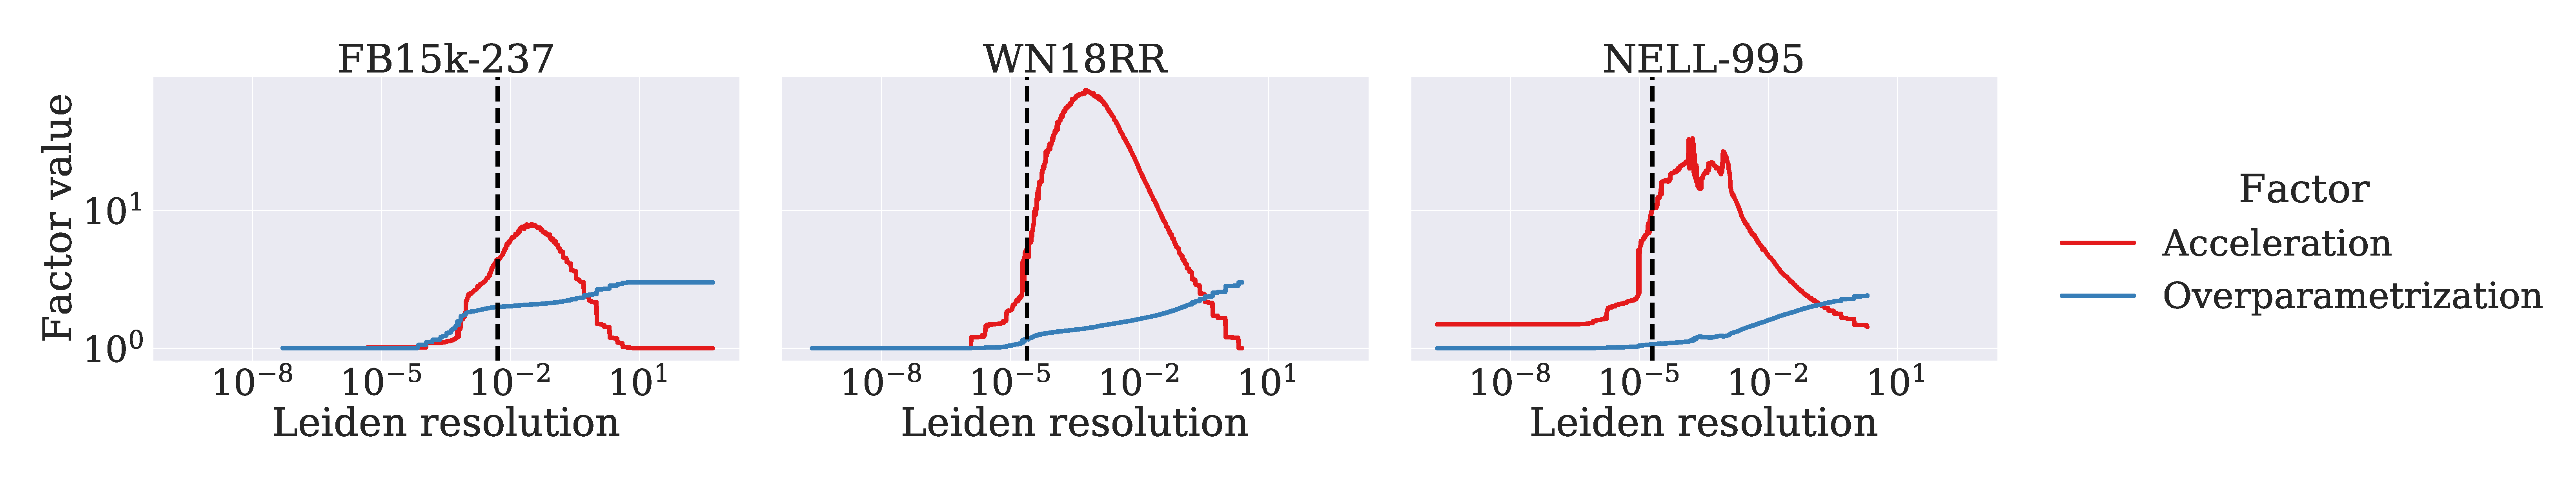
\includegraphics[width=\textwidth]{figures/coins/scalability_leiden_resolution}
\end{center}
\caption[Dependence of time and memory scalability on the value of the resolution hyperparameter of the Leiden community detection algorithm.]{Dependence of time and memory scalability (acceleration and overparametrization factors) on the value of the resolution hyperparameter of the Leiden community detection algorithm. Left to right: different datasets. Chosen hyperparameter values that yielded optimal balance between scalability and performance for each dataset annotated via vertical lines.}
\label{fig:scalability_resolution}
\end{figure}


% Figure~\ref{fig:scalability_cut_size} illustrates an alternative method to optimize the scalability factors, through optimization of the cut size (number of inter-community edges) heuristic utilized by the METIS algorithm. For Leiden, one observes smooth curves with similar properties as in Figure~\ref{fig:scalability_resolution}. For optimal acceleration, there seems to be a critical cut size, while having more inter-community edges implied more parameters for $f_*$. Curiously, we observed the METIS algorithm to yield a non-minimal cut size and there are a lot of Leiden resolution values that achieve lower cut sizes. METIS clearly favors too large of an increase in parameter number. The distribution of the metrics over a batch of 100 random uniform community assignments yielded extremal values: the best acceleration, however the largest cut size and most parameters.


% \begin{figure}[ht!]
% \begin{center}
% 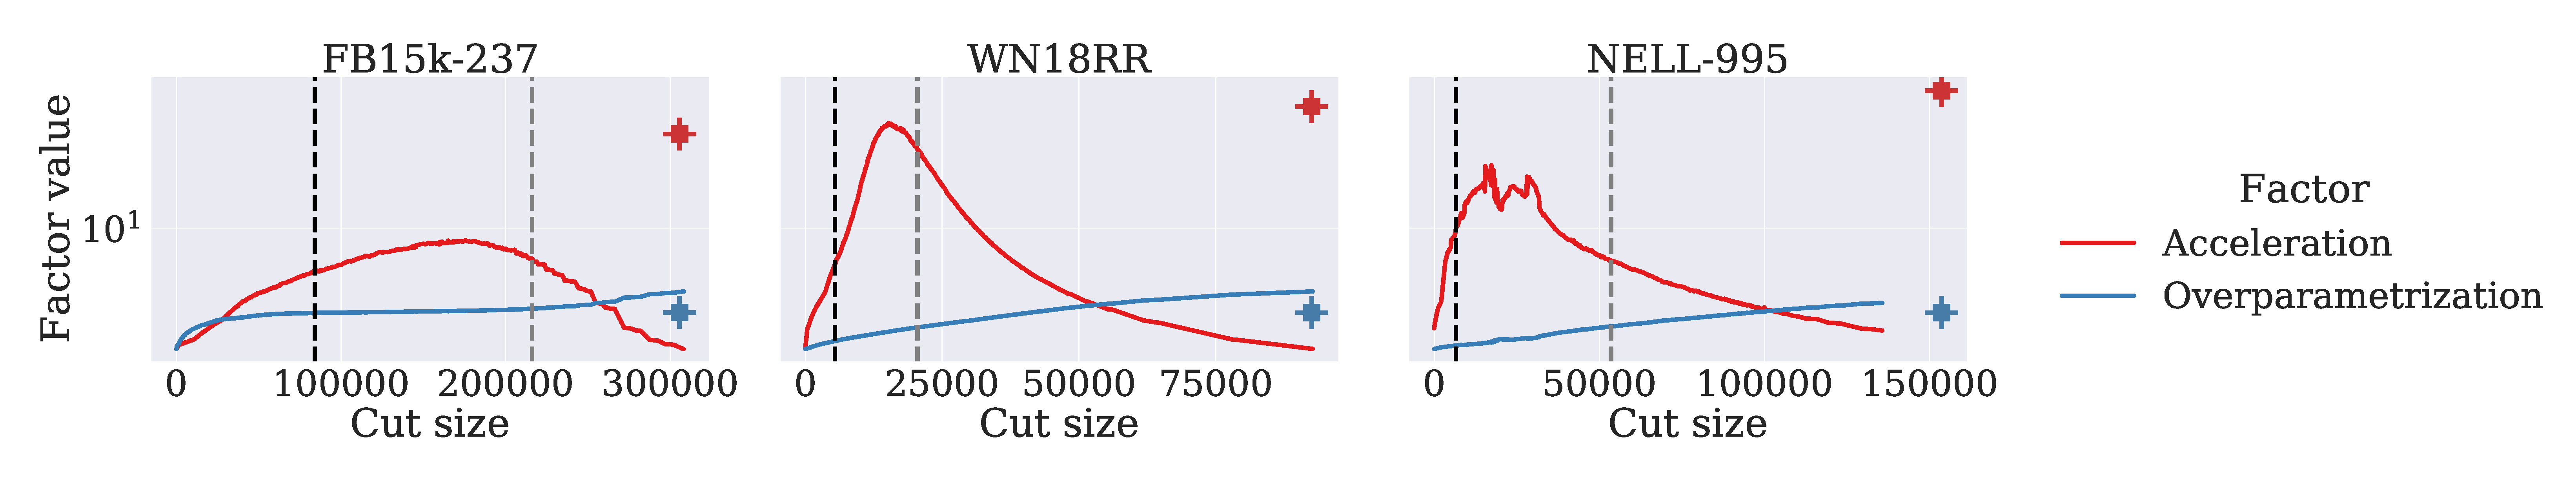
\includegraphics[width=\textwidth]{figures/scalability_leiden_cut_size}
% \end{center}
% \caption{Dependence of time and memory scalability (acceleration and overparametrization factors) on the cut size (number of inter-community edges) of community partitions obtained by varying the resolution hyperparameter of the Leiden community detection algorithm. Left to right: different datasets. Cut values that yielded optimal balance between scalability and performance for each dataset annotated via black vertical lines. Gray vertical lines denote the cut size values obtained by the METIS algorithm, while the boxes with error bars denote the results from a batch of 100 random uniform community assignments.}
% \label{fig:scalability_cut_size}
% \end{figure}

\subsubsection{Performance \& Feasibility}

Tables~\ref{tab:performance_query_answering_mrr} and~\ref{tab:performance_query_answering_q2b} contain our MRR metric query answering results and the comparison with the baselines, where KBGAT baselines were retrieved from~\cite{nathani_learning_2019}, Query2Box metrics were obtained by integrating the base algorithm with our experiment code that has COINs integration deactivated, while for all other models, metrics were calculated by running the implementation provided with~\cite{sun_rotate_2019}\footnote{Available at \url{https://github.com/DeepGraphLearning/KnowledgeGraphEmbedding}}. 
One can observe that on average, the relative error of the metric to the baseline decreases with the model complexity. This is to be expected, as more representation power means better embedding of the complicated community-node interactions. In a third of the single-hop cases and the majority of multi-hop ones, we even improve upon the baseline results.
%\clearpage

\begin{table}[H]
  \caption[Computed MRR metric of single-hop query answering experiments.]{Computed MRR metric (higher is better) of single-hop query answering experiments for comparison of COINs results to baselines with equal hyperparameters. Values in bold indicate the superiority of COINs, while underlined values have a relative error lower than 10\%.}
  \label{tab:performance_query_answering_mrr}
  \centering
\begin{tabular}{lllllll}
\toprule
Dataset & \multicolumn{2}{l}{FB15k-237} & \multicolumn{2}{l}{WN18RR} & \multicolumn{2}{l}{NELL-995} \\
Value &                 Baseline &                              COINs &                Baseline &                           COINs &                 Baseline &                           COINs \\
Algorithm &                          &                                    &                         &                                 &                          &                                 \\
\midrule
TransE    &              ${{0.218}}$ &            ${{0.132}_{\pm 0.004}}$ &              ${{0.16}}$ &  $\mathbf{{0.278}_{\pm 0.008}}$ &              ${{0.312}}$ &         ${{0.218}_{\pm 0.009}}$ \\
DistMult  &              ${{0.344}}$ &            ${{0.068}_{\pm 0.009}}$ &             ${{0.433}}$ &         ${{0.261}_{\pm 0.071}}$ &              ${{0.395}}$ &         ${{0.127}_{\pm 0.022}}$ \\
ComplEx   &              ${{0.369}}$ &     $\mathbf{{0.431}_{\pm 0.006}}$ &             ${{0.462}}$ &         ${{0.358}_{\pm 0.018}}$ &              ${{0.466}}$ &  $\mathbf{{0.472}_{\pm 0.005}}$ \\
RotatE    &              ${{0.383}}$ &  $\underline{{0.381}_{\pm 0.003}}$ &             ${{0.476}}$ &  $\mathbf{{0.487}_{\pm 0.001}}$ &              ${{0.482}}$ &         ${{0.412}_{\pm 0.018}}$ \\
KBGAT     &              ${{0.518}}$ &            ${{0.245}_{\pm 0.015}}$ &              ${{0.44}}$ &         ${{0.359}_{\pm 0.003}}$ &               ${{0.53}}$ &  $\mathbf{{0.543}_{\pm 0.009}}$ \\
% Query2Box &  ${{0.154}_{\pm 0.004}}$ &     $\mathbf{{0.261}_{\pm 0.002}}$ &  ${{0.26}_{\pm 0.001}}$ &  $\mathbf{{0.323}_{\pm 0.007}}$ &  ${{0.382}_{\pm 0.004}}$ &  $\mathbf{{0.443}_{\pm 0.004}}$ \\
\bottomrule
\end{tabular}
\end{table}

\begin{table}[H]
  \caption[Computed per-query-structure MRR metric of Query2Box query answering experiments.]{Computed per-query-structure MRR metric (higher is better) of Query2Box query answering experiments to compare our results with COINs training and evaluation to baselines with equal hyperparameters. Values in bold indicate the superiority of COINs, while underlined values have a relative error lower than 10\%.}
  \label{tab:performance_query_answering_q2b}
  \centering
    \begin{adjustbox}{width=\textwidth}   
\begin{tabular}{lllllll}
\toprule
Dataset & \multicolumn{2}{l}{FB15k-237} & \multicolumn{2}{l}{WN18RR} & \multicolumn{2}{l}{NELL-995} \\
Value &                 Baseline &                           COINs &                 Baseline &                              COINs &                 Baseline &                             COINs \\
Query &                          &                                 &                          &                                    &                          &                                   \\
\midrule
1p    &  ${{0.176}_{\pm 0.004}}$ &  $\mathbf{{0.276}_{\pm 0.003}}$ &  ${{0.258}_{\pm 0.004}}$ &     $\mathbf{{0.336}_{\pm 0.004}}$ &  ${{0.397}_{\pm 0.005}}$ &    $\mathbf{{0.463}_{\pm 0.009}}$ \\
2p    &  ${{0.027}_{\pm 0.001}}$ &  $\mathbf{{0.124}_{\pm 0.004}}$ &  ${{0.194}_{\pm 0.016}}$ &  $\underline{{0.182}_{\pm 0.026}}$ &  ${{0.516}_{\pm 0.033}}$ &    $\mathbf{{0.524}_{\pm 0.008}}$ \\
3p    &   ${{0.02}_{\pm 0.001}}$ &  $\mathbf{{0.117}_{\pm 0.008}}$ &  ${{0.141}_{\pm 0.009}}$ &      $\mathbf{{0.15}_{\pm 0.044}}$ &  ${{0.086}_{\pm 0.017}}$ &    $\mathbf{{0.172}_{\pm 0.022}}$ \\
2i    &  ${{0.091}_{\pm 0.008}}$ &  $\mathbf{{0.259}_{\pm 0.005}}$ &  ${{0.533}_{\pm 0.016}}$ &     $\mathbf{{0.668}_{\pm 0.025}}$ &  ${{0.313}_{\pm 0.063}}$ &    $\mathbf{{0.315}_{\pm 0.003}}$ \\
3i    &  ${{0.135}_{\pm 0.015}}$ &   $\mathbf{{0.303}_{\pm 0.01}}$ &  ${{0.913}_{\pm 0.151}}$ &         $\mathbf{{1.0}_{\pm 0.0}}$ &  ${{0.421}_{\pm 0.058}}$ &           ${{0.357}_{\pm 0.007}}$ \\
ip    &  ${{0.046}_{\pm 0.005}}$ &  $\mathbf{{0.188}_{\pm 0.008}}$ &  ${{0.329}_{\pm 0.068}}$ &            ${{0.193}_{\pm 0.029}}$ &  ${{0.487}_{\pm 0.029}}$ &           ${{0.278}_{\pm 0.033}}$ \\
pi    &  ${{0.039}_{\pm 0.004}}$ &   $\mathbf{{0.24}_{\pm 0.003}}$ &  ${{0.549}_{\pm 0.008}}$ &     $\mathbf{{0.609}_{\pm 0.075}}$ &  ${{0.585}_{\pm 0.073}}$ &  $\underline{{0.528}_{\pm 0.05}}$ \\
\midrule
Average &  ${{0.154}_{\pm 0.004}}$ &     $\mathbf{{0.261}_{\pm 0.002}}$ &  ${{0.26}_{\pm 0.001}}$ &  $\mathbf{{0.323}_{\pm 0.007}}$ &  ${{0.382}_{\pm 0.004}}$ &  $\mathbf{{0.443}_{\pm 0.004}}$ \\
\bottomrule
\end{tabular}
\end{adjustbox}
\end{table}

Refer to Tables~\ref{tab:performance_query_answering} and~\ref{tab:performance_query_answering_2} in Appendix~\ref{sec:appendix_results} for the full query answering metrics. 

To add further context to our obtained results, in Table~\ref{tab:performance_query_answering_related_work} we compared COINs-RotatE's performance to that reported by NodePiece~\cite{galkin_nodepiece_2022} and EARL~\cite{chen_entity-agnostic_2023}, the previously-mentioned related work that also provides scalable model-based solutions at the cost of some performance. From the table, we can infer that in all cases, our approach either beats the baseline or is the one that preserves the most of its strength.

\begin{table}[H]
  \caption[Comparison of Hits@10 and MRR values for query answering between the RotatE baseline, NodePiece, EARL and COINs.]{Comparison of Hits@10 and MRR values (averaged across seeds) for RotatE query answering between the baseline results in~\cite{sun_rotate_2019}, previous results by the related work NodePiece and EARL provided in~\cite{chen_entity-agnostic_2023} and this work. The top model is in bold, while the second best is underlined.}
  \label{tab:performance_query_answering_related_work}
  \centering
\begin{tabular}{lrrrr}
\toprule
{} & \multicolumn{2}{l}{Hits@10} & \multicolumn{2}{l}{MRR} \\
Dataset & FB15k-237 & WN18RR & FB15k-237 & WN18RR \\
Value     &           &        &           &        \\
\midrule
Baseline  &     \textbf{0.584} &  \underline{0.538} &  \textbf{0.383} &  \underline{0.476} \\
NodePiece &     0.420 &  0.515 &     0.256 &  0.403 \\
EARL      &     0.501 &  0.527 &     0.310 &  0.440 \\
COINs     &     \underline{0.552} &  \textbf{0.586} &     \underline{0.381} &  \textbf{0.487} \\
\bottomrule
\end{tabular}
% \begin{tabular}{lrrrrrr}
% \toprule
% {} & \multicolumn{2}{l}{MRR} & \multicolumn{2}{l}{Overparametrization} & \multicolumn{2}{l}{Ratio} \\
% Dataset & FB15k-237 & WN18RR &           FB15k-237 & WN18RR & FB15k-237 & WN18RR \\
% Value     &           &        &                     &        &           &        \\
% \midrule
% Baseline  &     0.383 &  0.476 &               1.000 &  1.000 &     0.383 &  0.476 \\
% NodePiece &     0.256 &  0.403 &               1.103 &  1.073 &     0.232 &  0.376 \\
% EARL      &     0.310 &  0.440 &               0.621 &  0.927 &     0.499 &  0.475 \\
% COINs     &     0.381 &  0.487 &               1.995 &  1.165 &     0.191 &  0.418 \\
% \bottomrule
% \end{tabular}
\end{table}

However, a relevant comparison to the baseline is difficult to perform without the aid of an additional scalability-dependent investigation of the applicability of our proposed approach. Unlike~\cite{chen_entity-agnostic_2023}, which only evaluated the ratio of absolute MRR to model size, we believe the more direct and robust scalability comparison is one between the relative error and speed-up. Thus, we plot our values for the relative error in MRR to the baseline against acceleration (reduction in computational complexity) in Figure~\ref{fig:feasibility}. 

\begin{figure}[H]
\begin{center}
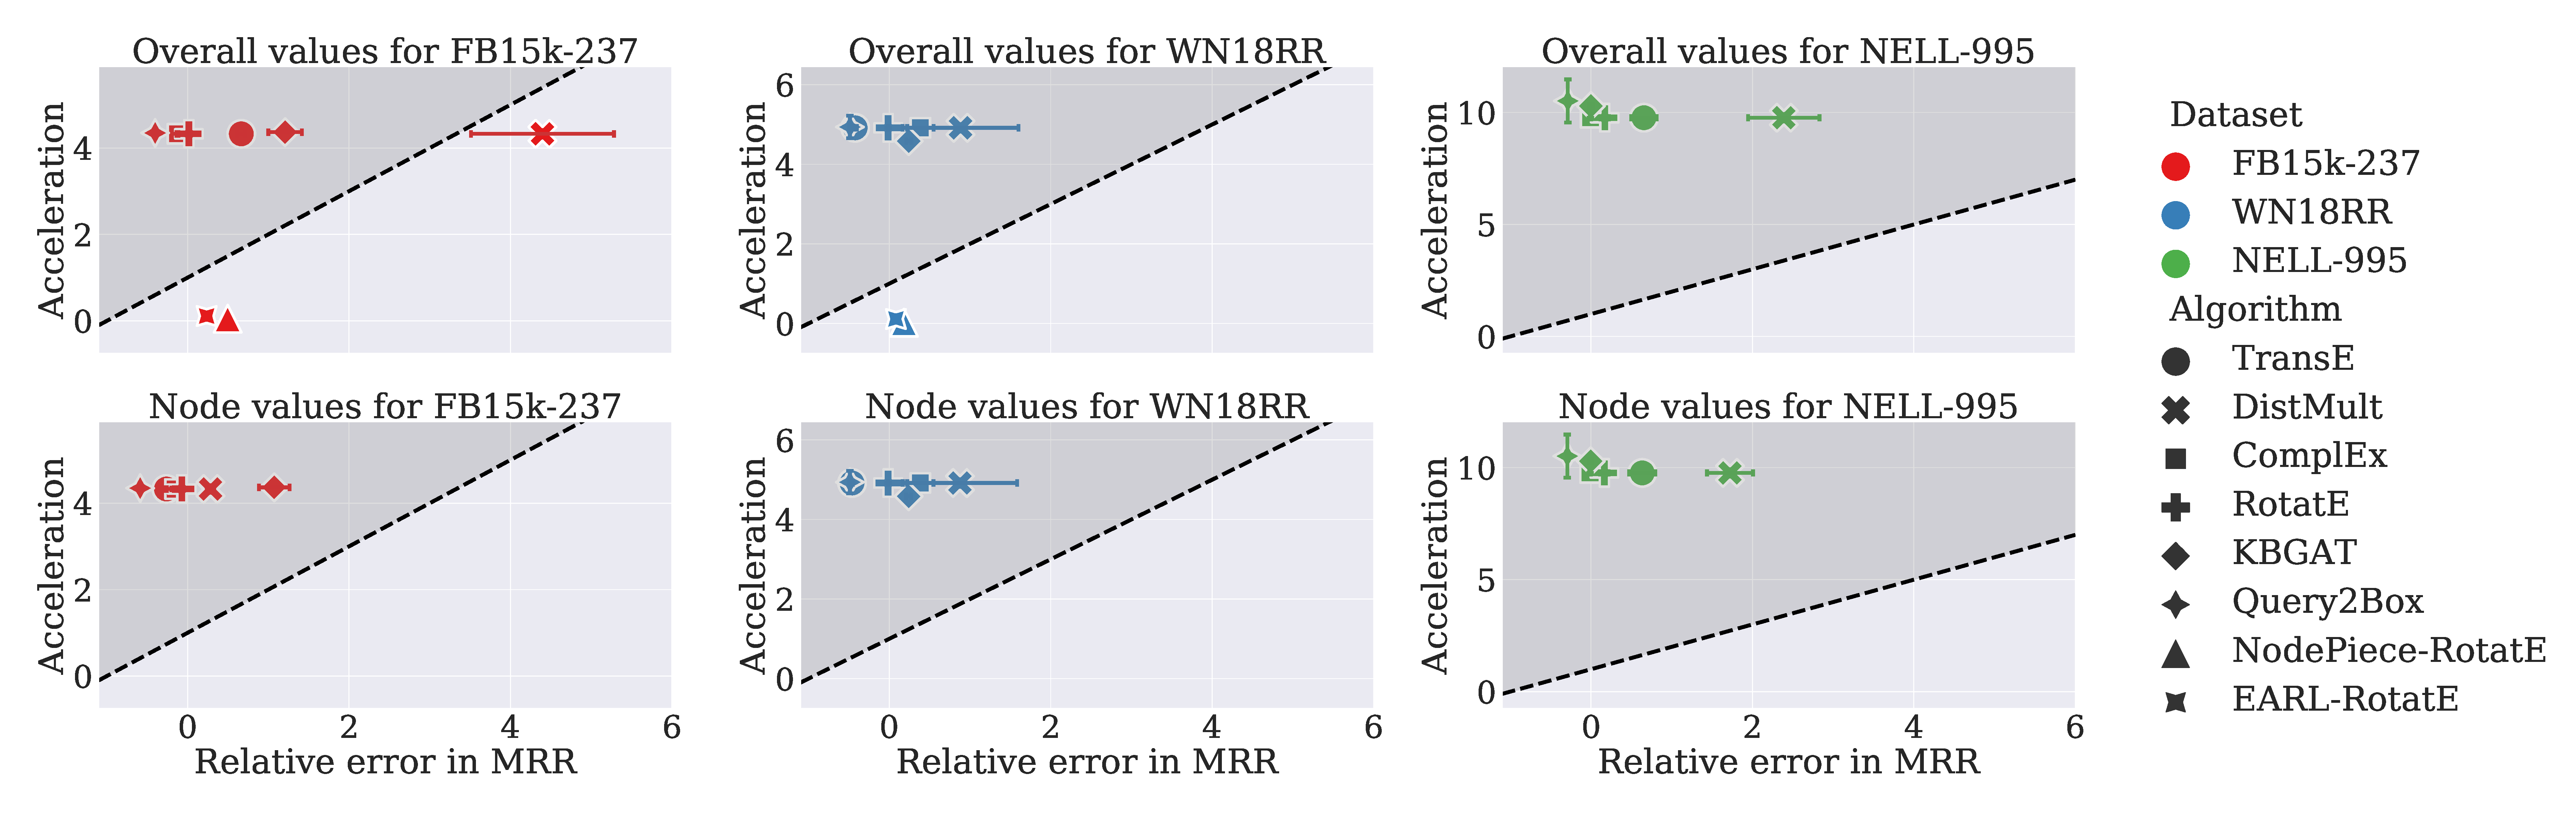
\includegraphics[width=\textwidth]{figures/coins/feasibility_2.pdf}
\end{center}
\caption[Plot of relative error in MRR against acceleration.]{Plot of relative error in MRR (lower is better) against acceleration (higher is better). The feasible region is the one shaded, where the speed-up is by at least 100\% larger than the error. Top vs. bottom: values computed from ranks after both steps vs. just the second step of COINs. Removing the error in the ranks caused by the community prediction shows improvement and feasibility of all experiments, explaining the outliers, i.e. some models' inability to learn Freebase communities well. Left to right: different datasets.}
\label{fig:feasibility}
\end{figure}

From the top plots, one can observe that almost all COINs experiments lie deep in the feasible region, with the bottom plots explaining the reason for the few outliers. On the other hand, the NodePiece and EARL baselines are made infeasible by the time-memory trade-off of tokenization.

\subsection{Summary}

In this section we introduced COINs, a method for accelerating link prediction and query answering models for knowledge graphs, to be applicable even in low computational resource settings. COINs featured a two-step prediction procedure: query answer prediction via community prediction and within-community localization. 
% This first answer localization step was found to be very impactful on overall model performance. 
We theoretically and empirically elaborated that the quality of the community structure of the knowledge graph has a broad-reaching influence on the possible scalability improvements provided by our method, as well as its prediction performance compared to baselines. As such, one can conclude that before selecting COINs to accelerate the embedding of a knowledge graph, it is important to study and evaluate its community structure. 

The achieved impressive accuracy and acceleration benefits strongly motivate modeling and predicting over both the community-level coarsened version of a knowledge graph in addition to the local structures, no matter the task. We would in such a way, apply both holistic and reductionist techniques to solve a knowledge graph problem, perhaps otherwise computationally intractable.

As relevant future work in scalable knowledge graph reasoning, we propose attempting the integration of COINs with algorithms for general first-order logical knowledge graph query answering, like BetaE~\cite{ren_beta_2020}, and obtaining comparisons to baseline models on larger non-standard knowledge graphs.